\chapter{Bilan et perspectives}
\label{chap:bilan}

\section{Organisation du travail}
\label{sec:orga}
  \subsection{Application du référentiel qualité interne}
  \label{sec:qualite-interne}

  Nous exposons ici les éléments fournis par SII ayant guidé de manière significative la conduite du projet. 
  Ceux-ci seront plus ou moins détaillés en fonction du temps consacré à leur mise en place.
  
    \begin{figure}[h]
    \centering
      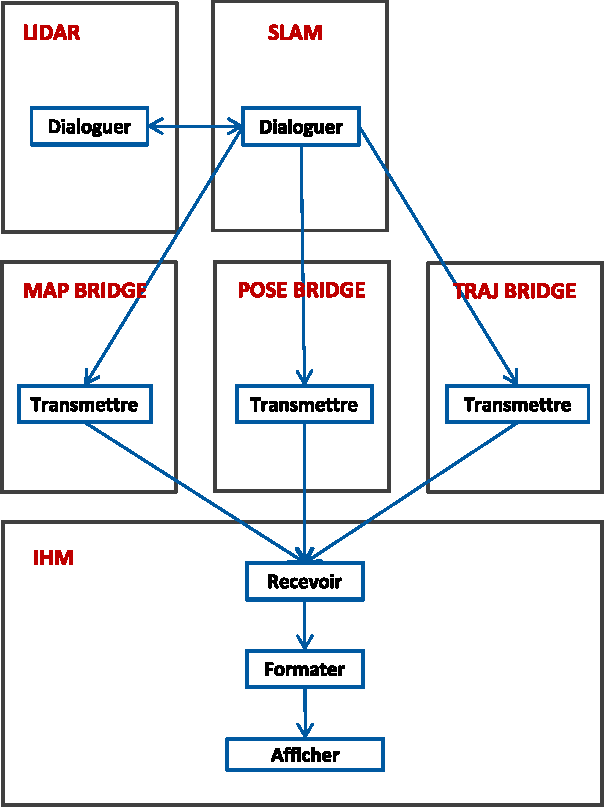
\includegraphics[width=.6\linewidth]{figures/rel-fonctions}  
    \captionof{figure}{Modèle de définition des modules logiciels et relations entre leurs fonctions}
    \label{fig:rel-fonctions}
  \end{figure}
  
  Les premiers éléments oraganisationnels qui ont été formalisés s'incarnent par deux documents de spécification appelés \gls{STBL} et \gls{DCL}.
  Le premier vise, comme son nom l'indique, à exprimer le plus objectivement possible le besoin qui justifie la réalisation logicielle, notamment au moyen d'exigences représentées figure \ref{fig:exigences}. 
  Cette énumération haut-niveau permet d'appréhender simplement et rapidement le périmètre du logiciel ciblé. 
  Cependant, la réalisation de ce document en bonne et dûe forme nécessite une liste exaustive d'exigences fonctionnelles vues comme des ensembles de fonctions qu'il convient de décrire en terme de rôle, d'entrées, de sorties et
  de traitements. 
  Dans le cadre de ce stage, nous définissons des fonctions comprises dans des modules distincts et étant reliés comme présenté sur la figure \ref{fig:rel-fonctions}.
  Puis, pour chacune des fonctions, on va définir des sous-fonctions, idéalement jusqu'à un niveau de granularité maximal où tous les types de données sont énumérés. 
  Par exemple, on établit que la fonction \emph{Transmettre} du module \textbf{\textcolor{red-stbl}{Map\_bridge}} regroupe les trois sous-fonctions \emph{Recevoir un message}, \emph{Formater un message} et \emph{\'{E}mettre un message}. 
  Afin d'illustrer cette démarche, nous donnons ici pour exemple la spécification de la fonction \emph{Transmettre : Formater un message}. 
  
  \textbf{1. Rôles } \\
  Cette fonction est activée à l’arrivée d’une demande de traitement de message sur la liaison SLAM $\Longleftrightarrow{}$ MAP\_BRIDGE.
  Elle intervient après que la fonction de réception ait attesté de la consistance du message reçu.
  Elle permet d’extraire la charge utile du message reçu et d’en réduire significativement le volume avant envoi.  Les données en sorties sont sérialisées.
  Cette extraction s’effectue en comparant OCCUPANCY\_GRID avec une copie locale de la dernière carte reçue OLD\_OCCUPANCY\_GRID.
  
  \textbf{2. Entrées }
  \begin{figure}[!h]
    \begin{center}
      \begin{tabular}{|l|l|}
	\hline
	\textbf{Désignation} & \textbf{Type de données} \\
	\hline
	Message OCCUPANCY\_GRID & OccupancyGrid \\
	\hline
      \end{tabular}
    \end{center}
    \caption{Entrées de la fonction \emph{Transmettre : Formater un message}}
  \end{figure}
  
  \textbf{3. Sorties }
  \begin{figure}[!h]
    \begin{center}
      \begin{tabular}{|l|l|}
	\hline
	\textbf{Désignation} & \textbf{Type de données} \\
	\hline
	Message MAP & OccupancyGridUpdate \\
	Message INI\_MAP & IniOccupancyGrid \\
	\hline
      \end{tabular}
    \end{center}
    \caption{Sorties de la fonction \emph{Transmettre : Formater un message}}
  \end{figure}
  
  Notons que la spécification des types de données d'entrées-sorties est donné dans un document externe. 
  Relativement à l'exemple précédent, le type d'OCCUPANCY\_GRID est décrit en \nameref{annexe:occupancygrid}.  
  
  \textbf{4. Traitements }
  
  \textbf{NB} : Les traitements sont idéntifiés de manière unique au sein d'un document, ils satisfont également des règles permettant d'être traités automatiquement par des logiciels de suivi de projet. 
  Nous donnons ici un exemple succint permettant d'en saisir le sens. Dans la pratique une sous-fonction donne lieu à plusieurs traitements.
  
  \textbf{$[$REQ\_STBL\_MAP\_BRIDGE\_FORM\_1$]$}
  
    \hspace{10mm} Si OLD\_OCCUPANCY\_GRID existe : 
    
    \hspace{10mm} On compare le champ ``data'' de OCCUPANCY\_GRID et de 
    \\ OLD\_OCCUPANCY\_GRID. 
    
    \hspace{10mm} On crée la structure MAP à partir des valeurs de ``data`` qui diffèrent. 
    
    \hspace{10mm} MAP est une chaîne de caractères dont les valeurs sont séparées par des ",".\\ 
  \textbf{$[$FIN\_REQ$]$}
  
  Le Document de Conception Logicielle est quant à lui intervenu plus tard dans l'avancée du stage. 
  Il consiste à formaliser les éléments conceptuels, en termes d'architecture physique et logicielle du projet. 
  Ces briques ayant été largement explicitées au long de ce rapport nous n'étayerons pas d'avantage ce point. 
  
  Un planning présentant une granularité hebdomadaire a été effectué au mois de mars, ce document est présenté en \nameref{annexe:planning}.
  Cette réalisation vise d'une part à définir et ordonnancer les tâches à réaliser et, d'autre part, à estimer l'impact temporel de chacune d'entre-elles. 
  Ce document a été réalisé dans une optique d'organisation personnelle mais a également constitué un outil d'évaluation et de communication avec M. Daumand qui a été en grande partie affecté en missions hors de l'agence. 
  Il s'agissait donc pour nous de fixer les jalons clés, les \emph{dead-lines} et les versions du logiciel à produire afin qu'il suive de manière pragmatique l'avancée du travail. 
  
  \subsection{Vers une conduite AGILE adaptée}
  
  Au référentiel interne de qualité du logiciel se sont ajoutées certaines bonnes pratiques issues de la formation en Architecture et Sécurité du Logiciel prodiguée à l'INSA Centre Val-de-Loire.
  En particulier, nous avons utilisé le gestionnaire de versions Git au travers du système de gestion de dépôts (forge) GitLab auquel nous avons appliqué une stratégie de création de branches dite \og Git Flow \fg{}.
    \begin{figure}[h]
    \centering
      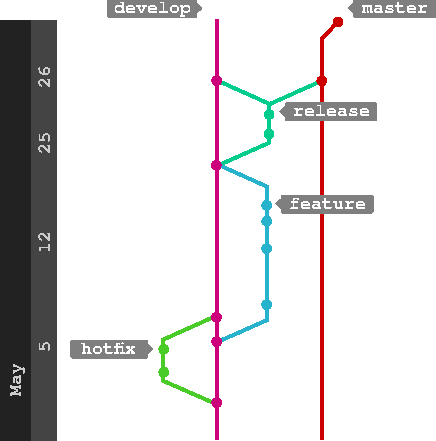
\includegraphics[width=.6\linewidth]{figures/gitflow}  
    \captionof{figure}{Politique de gestion de branches Git adoptée}
    \label{fig:gitflow}
  \end{figure}
  Ce modèle d'utilisation de Git vise à minimiser les conflits et les régressions, accentuer la visibilité des tâches en cours ou terminées et à scinder clairement les phases de développement du logiciel. 
  \`{A} cet effet nous avons adopté la démarche illustrée sur la figure \ref{fig:gitflow} qui se lit de bas en haut et où les commits sont représentés par des points.
  Cela consiste à travailler sur une branche de développement (\path{develop}), à partir de laquelle nous créons une branche par fonctionnalité (\path{feature}), éventuellement une branche \path{hotfix} pour une correction de bug
  et, enfin, une branche \path{realease} qui va aboutir sur la dernière version stable du logiciel.
  Cette branche est ensuite répercutée sur \path{develop} et \path{master}, dans le premier cas  pour continuer les actions de développement et dans le second, afin de permettre la récupération des sources ou leur déploiement. 
  
  Aussi, l'\path{Apploader} a constitué une refonte majeure de l'architecture du logiciel qui a été conceptualisée et développée en équipe. 
  Afin de répartir les tâches que nécessitait son implémentation, nous avons pu expérimenter l'utilisation d'un \gls{Kanban} recensant : 
  
  \begin{itemize}
   \item les tâches à effectuer, par exemple \emph{Enregister les données de cartographie dans le format DOG}
   \item la complexité relative de chacune d'entre-elles 
   \item les dépendances de certaines tâches les unes par rapport aux autres
  \end{itemize}

  Définir la \og complexité \fg{} d'une tâche revient à lui attribuer un score en se référant aux scores attribués pour les tâches précédentes. 
  Les méthodes AGILES --notamment \gls{SCRUM}-- préconnisent le recours à des échelles de quantification relatives plutôt qu'à des jours hommes ou d'autres échelles se voulant précises. 
  Concrètement on peut utiliser les valeurs de la suite de Fibonacci qui suivent ce que l'on appelle la courbe d'incertitude, à savoir qu'au plus une valeur est élevée, au plus l'écart avec la valeur suivante sera grande. 
  Nous avons estimé la complexité des unités de travail à réaliser selon une méthode également empruntée à SCRUM, appelée \emph{planning poker}. 
  Tous les participants disposent d'un jeu de carte qui, dans notre cas, comporte les nombres $\dfrac{1}2, 1, 2, 3, 5, 8, 13, \infty$. 
  L'effort de réalisation est ensuite estimé en même temps pour une tâche donnée, puis soumis à discussion dans le cas de désaccord. 
  Cette pratique est à la fois rapide, ludique et présente l'intérêt de dénuer d'emblée la quantification de l'influence mutuelle des participants. 
  
  Ce Kanban a ainsi été adopté dans une optique d'ordonnancer les tâches et, accessoirement, de les répartir entre les membres de l'équipe. 
  Il a aussi permis d'attester visuellement de nos avancées respectives et du nombre de tâches en cours permettant un allègement ou une répartition de la charge si besoin.
  La consultation du nombre de tâches restantes a également joué dans nos décisions de poursuivre telle ou telle fonctionnalité au profit d'autres. 
  
\section{Résultats en vue d'un prolongement}  
  \subsection{Un module de SLAM en adéquation avec les attentes du projet}
  
  Nous nous intéressons dans un premier temps à la fidélité des résultats de SLAM et ensuite à une appréciation de l'ensemble du projet, incluant également les travaux d'Alban Chazot et bien sûr la vision de M. Daumand.  
  
  La figure \ref{fig:carto} donne un aperçu de la précision des résultats de SLAM. 
  Elle met en parallèle les résultats cartographiques du système avec un plan d'évacuation des locaux dans lesquels l'acquisition a pu être menée. 
  Pour des raisons pratiques, toutes les pièces n'ont pu être scannées, puisque celles-ci hébergent des collaborateurs ou directeur d'agence menant leurs activités.
  
  \begin{figure}[h]
    \centering
      \includegraphics[width=1.\linewidth]{figures/plan}  
    \captionof{figure}{\`{A} gauche cartographie des locaux avec le logiciel, à droite plan d'évacuation correspondant}
    \label{fig:carto}
  \end{figure}
  
  Le plan des locaux est complété par des cercles de couleur verte pour les pièces qui ont été au moins à moitié explorées et de couleur orange pour les pièces visibles à moins de $50\%$. 
  Enfin nous représentons sur fond gris les pièces qui n'ont pas été scannées du tout. 
  Le couloir central a été parcouru dans toute sa longueur et la porte d'entrée est pointée par une flèche noire sur les deux représentations, afin d'éviter toute confusion quant à la façon de les interpréter. 
  
  On remarque empiriquement que les lieux cartographiés sont reconnaissables sans trop de difficultés, que leur agencement correspond à la réalité perçue et que les proportions des salles sont pour la plupart fidèles. 
  On peut aussi noter la précision du rendu des obstacles fixes : portes, pieds de tables, de chaises ou du baby-foot situé au centre de l'accueil dont trois pieds sur quatre sont visibles et correctement situés. 
  La géométrie des murs est également respectée, ce qui peut être attesté par les angles droits des pièces ou la régularité du couloir. 
  
  Cependant le résultat n'est pas sans défauts et certaines erreurs méritent d'être discutées. 
  L'imperfection la plus flagrante se situe au niveau du bureau 2. 
  Selon la cartographie celui-ci est aussi long que le bureau 3, tandis qu'il est, dans les faits, presque deux fois plus long. 
  Cette déformation se retrouve en effet sur toutes les acquisitions qui se sont déroulées de la manière suivante : 
  \begin{itemize}
   \item départ du bureau 3
   \item sortie du bureau 3 en direction du bureau 2
   \item déplacement dans un couloir de 8 mètres
   \item arrivée dans le bureau 2
  \end{itemize}

  Lorsque la plateforme longe le couloir, le moteur de SLAM est confronté à une problématique typique : les points de repères extraits sont les mêmes à des temps et positions différentes. 
  En effet, il n'est pas possible d'extraire des caractéristiques spatiales autres que des murs droits, jusqu'à ce que l'entrebaillement de la porte du bureau 2 ne soit visible. 
  Dans ce cas, l'association de données interne au processus de SLAM va fusionner les repères perçus à différents points de la zone traversée, générant des erreurs de cartographie et de localisation.  
  Ce phénomène est observable lors du téléguidage du robot à travers le couloir, \gls{Hector SLAM} va retourner des positions successives identiques sur quelques mètres alors que la position réelle du robot a évolué.
  La zone bleue sur le plan d'évacuation représente la portion de l'espace parcouru sur laquelle \gls{Hector SLAM} a estimé que la plateforme faisait du \og sur-place \fg{}. 
  
  Une réponse à cette problématique pourrait être de se fier davantage à l'odométrie, puisque les encodeurs des roues du robot détiennent l'information jusqu'ici manquante : le robot a avancé ou reculé. 
  Or Hector SLAM a été choisi spécifiquement pour sa faculté à se baser en priorité sur les données issues du LIDAR. 
  Ce moteur de SLAM présente donc des limites intrinsèques pour une utilisation dans des environnements lisses, où peu de repères spatiaux évidents sont perceptibles.  
  L'amélioration des résultats dans notre couloir reviendrait à utiliser un LIDAR à plus grande portée, capable de déceler des caractéristiques plus lointaines
  \footnote{On rappelle que la portée maximale du RPLidar A2 est de $6m$.}.
  
  Enfin, la réussite du projet dans sa globalité a pu être attestée par les résultats d'une présentation devant des collaborateurs commerciaux et directeurs de projet qui est intervenue le 13 juin 2017.
  Cette étape a permis de reccueillir des avis extérieurs sur le projet lui-même et d'estimer sa potentielle viabilité commerciale et technique. 
  Ayant été positivement perçu, le système démonstrateur réalisé a été présenté brièvement auprès d'interlocuteurs de Nexter Systems, enclins à organiser une rencontre à cet effet au mois de septembre. 
  
  \subsection{Pourquoi et comment envisager la continuité de SRT2M ?}
  
  La présentation du projet à un client tel que Nexter Systems étant un objectif établi depuis la phase d'analyse préliminaire, nous avons veillé à maximiser le potentiel d'appropriation de ce dernier par de tierces personnes.
  Cette volonté s'est incarnée par la mise en place des éléments suivants : 
  
  \begin{itemize}
   \item un manuel utilisateur interactif et ergonomique présenté au sein d'une interface web
   \item un manuel d'installation, agrémenté de résolutions problèmes pouvant être rencontrés lors de cette phase
   \item la création d'une documentation automatique et, là aussi, interactive grâce au logiciel Doxygen
   \item l'automatisation de l'installation pour la distribution Debian 8, notamment au moyen du gestionnaire de paquets apt, et la gestion des dépendances manquantes sur la station hôte
   \item l'adoption de ROS répondant à un critère de haute flexibilité fonctionnelle et matérielle
   \item l'adaptation des possibilités de l'IHM au caractère modulaire des éléments du middleware ROS 
  \end{itemize}
  
  
  Par ailleurs, ce projet mené de bout en bout a suscité un foisonnement d'idées applicatives, dont nous rappelons ici le scénario majeur : une application militaire facilitant l'accès à des informations stratégiques. 
  Tout d'abord, la mise en \oe{}uvre d'algorithmes de SLAM aboutit généralement sur des systèmes capables de naviguer en autonomie ou semi-autonomie. 
  Moyennant une adaptation du matériel à cet effet, cette fonctionnalité peut être atteinte rapidement. 
  Elle constitue aussi un pré-requis aux applications envisagées. 
  
  \begin{figure}[h]
    \centering
      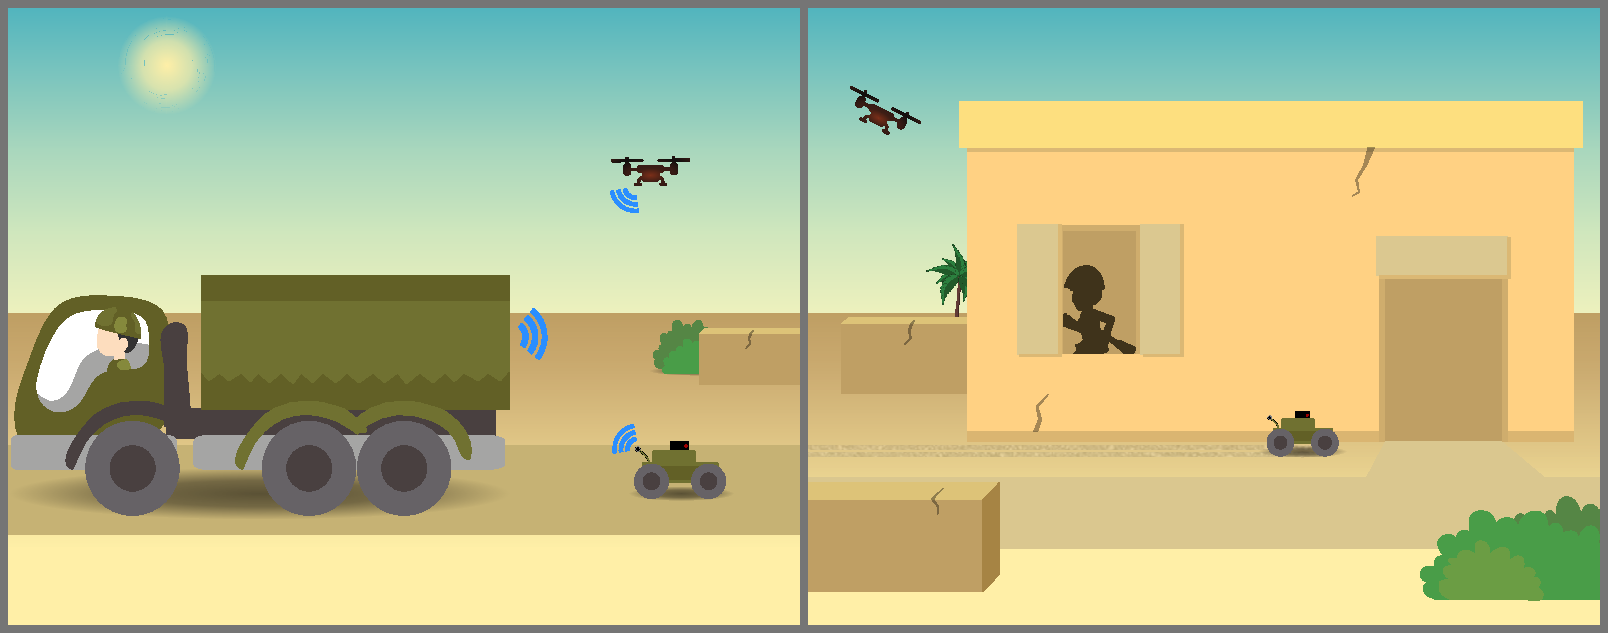
\includegraphics[width=1.\linewidth]{figures/ml_collage}  
    \captionof{figure}{Illustration : déploiement et approche furtive de la flotte}
    \label{fig:srt2M-1}
  \end{figure}
  
  Le scénario principal que nous cherchons à illustrer ici est composé d'une flotte de véhicules autonomes, à la fois aériens et terrestres, pilotés à distance par un opérateur (voir figure \ref{fig:srt2M-1}). 
  Le système logiciel embarqué est distribué sur chacun des terminaux mobiles, chacun d'entre-eux étant atteignable par ondes radio ou WiFi sur un canal de communication chiffré. 
  L'opérateur va émettre un ordre de mission correspondant à une zone à explorer, une niveau de furtivité et un temps imparti comprenant l'aller et le retour des modules.
  Une unité maîtresse sera responsable de la répartition des trajectoires à emprunter pour l'ensemble de la flotte, tandis que les calculs peuvent être répartis ou centralisés sur une station de travail abritée.
  Si le véhicule maître est indisponible ou défectueux, une autre unité endosse son rôle immédiatement. 
    \begin{figure}[h]
    \centering
      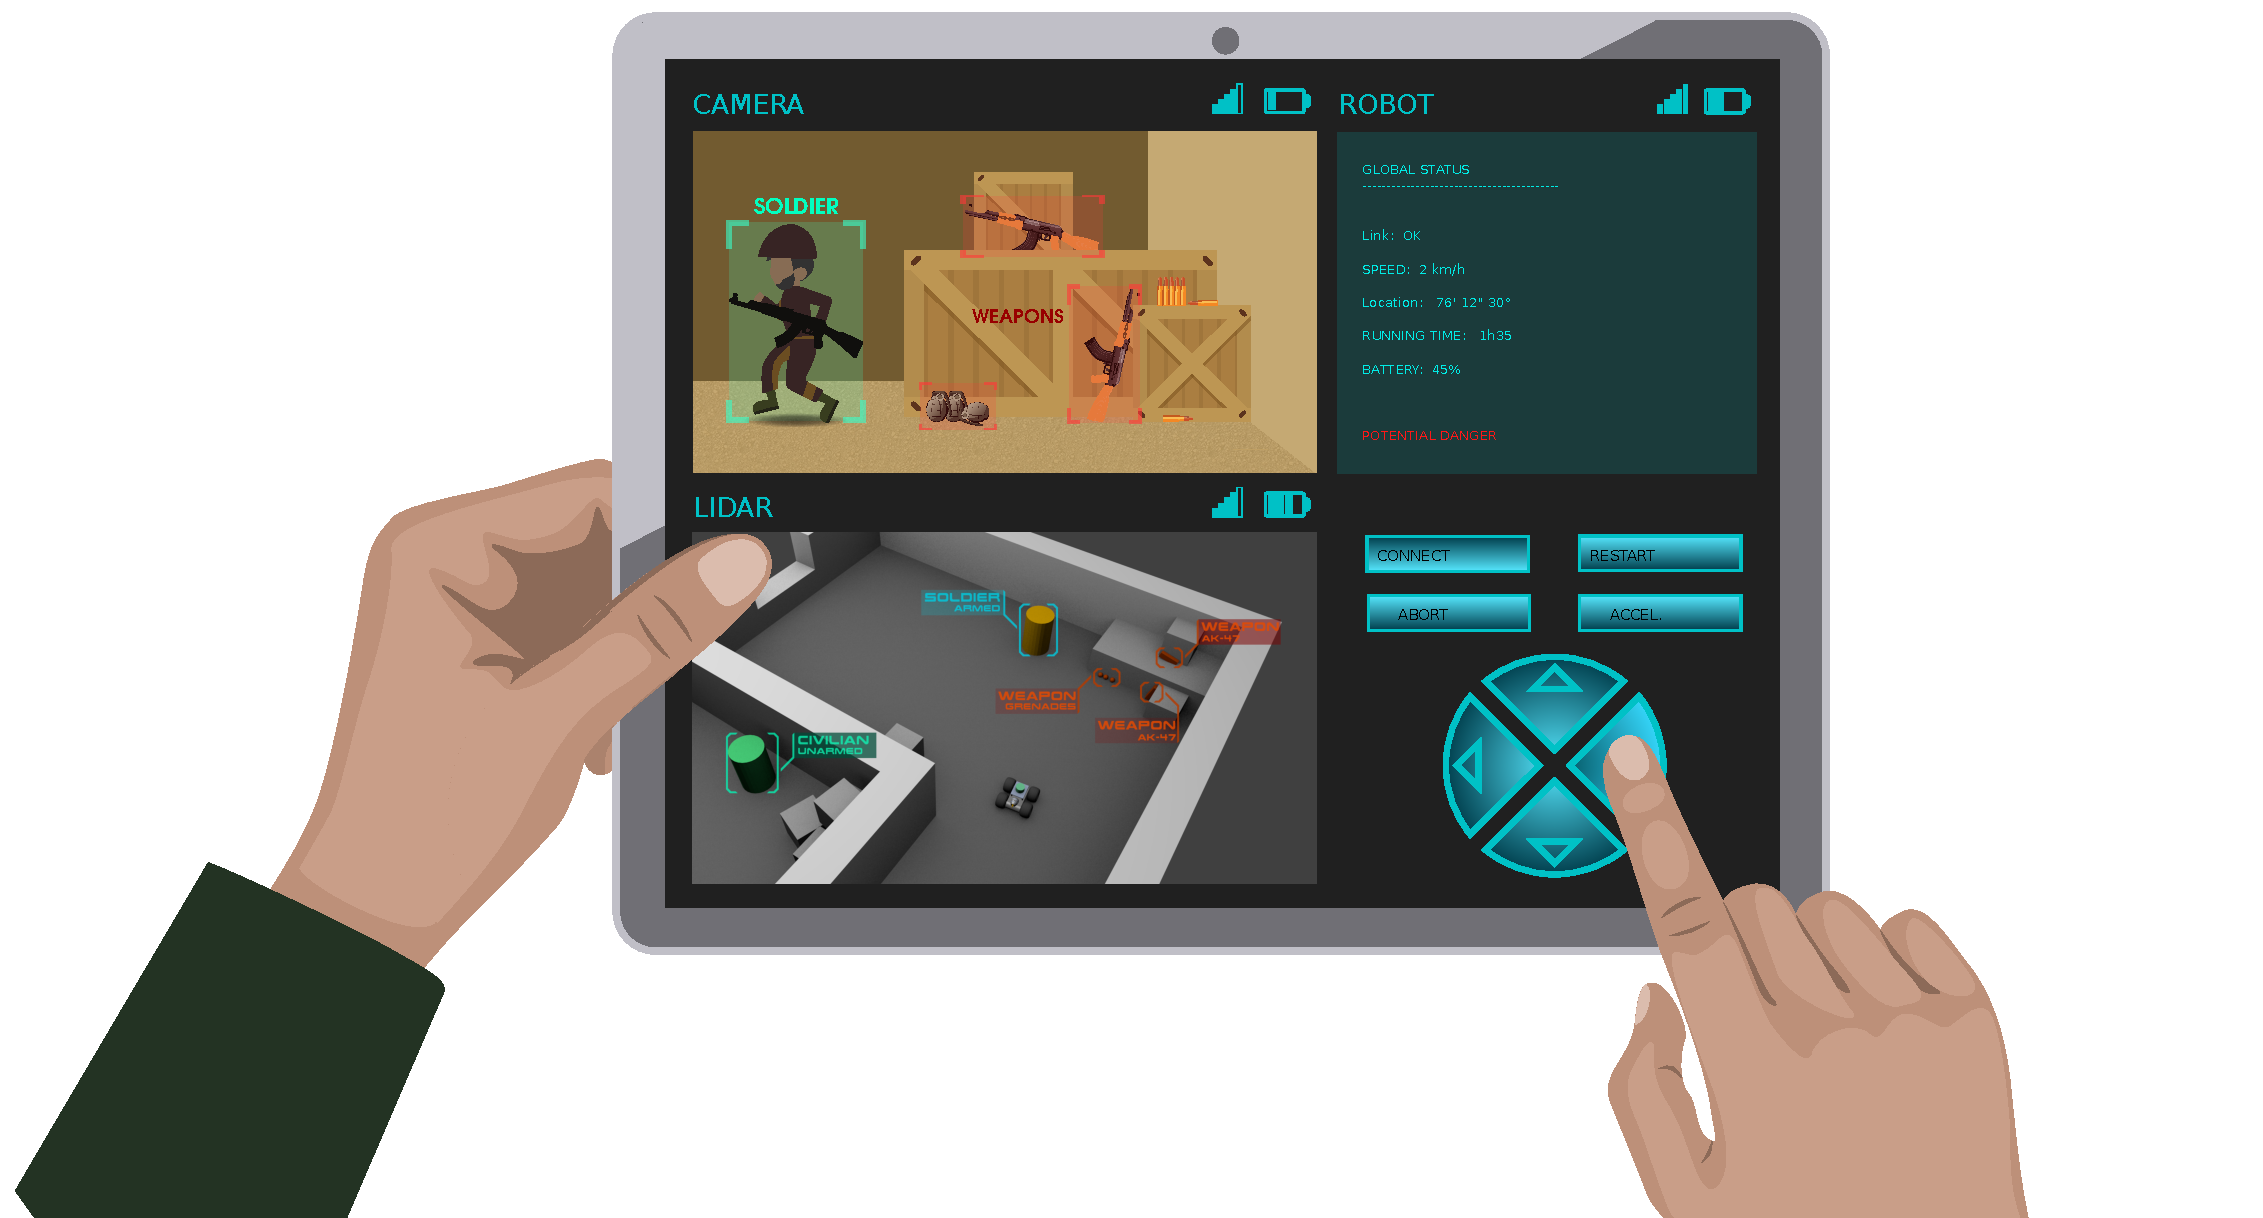
\includegraphics[width=1.\linewidth]{figures/ml_4}  
    \captionof{figure}{Illustration : réception de données unifiées}
    \label{fig:srt2M-2}
  \end{figure}
  La réception des données (figure \ref{fig:srt2M-2}) sera quant à elle unifiée en une seule cartographie permettant un prise en compte globale des jeux de données reçues. 
  
  On peut également envisager l'immersion du système dans des environnements qualifiés de \gls{USAR}.  
  Comme beaucoup d'applications robotiques issues du framework ROS, \gls{Hector SLAM} a été éprouvé lors de compétitions dédiées à la recherche de victimes. 
  Dans ce cas, il convient de définir quelles sont les situations de secourisme ciblées par le système : incendie, raz-de-marée, expositions radio-actives ou à d'autres substances toxiques ? 
  La réponse à ces questions permettra d'évaluer le coût du matériel adapté à ces scénarios ainsi que les temps de recherche, spécification, développement et tests susceptibles d'assurer un nouveau produit minimum viable. 
  
\section{Retour d'expérience}
  \subsection{Apports et difficultés du projet}
  
  Ce projet s'est trouvé complexe et stimulant à tous les niveaux. 
  Les phases de spécification du besoin ont été fastidieuses tant du fait de la rigueur des documents requis qu'au regard de mon manque de vision intial et de ma difficulté à me représenter ce que serait le système en bout de stage. 
  Cela s'explique notamment par une méconnaissance initiale du domaine de la robotique et du secteur de la défense.
  Les aides conjointes de MM. Daumand et Hafiane, de vastes recherches documentaires et un intérêt certain pour ce sujet où tout était à construire ont fort heureusement motivé une rapide appropriation des problématiques et enjeux afférents. 
  
  Les outils utilisés tels que ROS et à plus faible mesure Qt, ou les fondements théoriques du SLAM puis d'Hector SLAM ont également nécessité des temps de compréhension et d'assimilation conséquents. 
  Bien que n'ayant pas outrepassé le temps imparti à la recherche de solutions techniques, il m'est avéré difficile de passer plusieurs semaines à approfondir des connaissances très spécifiques --comme dans le cas de ROS-- sans 
  avoir la moindre idée de ce que donneront les débuts de l'implémentation. 
  Cet effet tunnel s'est trouvé renforcé du fait des délais d'acquisition du matériel et des incertitudes liées au fonctionnement du robot. 
  
  Aussi, nous avons eu la chance d'appréhender la réalisation d'un système à naître, sans qu'aucune étude préalable n'ait été menée. 
  Ce point a à la fois constitué un atout majeur dans le choix de ce stage, mais également une incertitude indéniable qui a compliqué la visualisation du système final. 
  Par exemple, la quantification précise du temps alloué aux diverses étapes de conception ou de réalisation s'est révélée être une pratique nouvelle et à la fois primordiale pour mener à bien ce genre de projets. 
  Ces difficultés ont peut-être avant tout été surmontées par la communication au sein de l'équipe, permettant de désamorcer les situations de doutes et de consolider sereinement une vision du projet à moyen terme. 
  
  Enfin, j'ai particulièrement apprécié l'alternance entre une période assez longue de travail individuel, et un travail en équipe --certes restreinte-- dans une seconde phase du développement. 
  Dans le premier cas, cela force à une organisation, une prise de décisions et de responsabilités individuelles accrues qui n'ont que très peu été expérimentées lors de projets scolaires au long-cours.
  Le deuxième temps de développement avec Alban Chazot a permis l'expérimentation d'outils issus de méthodes AGILES et adaptés à notre équipe minimale.  
  Cette deuxième phase s'est faite sur un ton plus détendu, les fonctionnalités primordiales du système ayant été présentées et validées. 
  
  \subsection{\'{E}volution personnelle au sein de la structure}
  
  Bien qu'elle soit inclue dans un groupe international, l'agence SII Bourges affiche un \og esprit \emph{startup}\fg{} indéniable. 
  L'équipe sur place est à taille humaine, d'une moyenne d'âge située autour d'une trentaine d'années et présente des normes décontractées soutenues par une hiérarchie horizontale.
  La société SII dénote d'une envie de séduire les plus jeunes actifs en brevetant le slogan \#FUNgenieur qui vise à \emph{``dépoussiérer l'image du geek austère''}, en proposant salles de jeu, de sport ou de détente dans ses agences et, 
  finalement, en misant sur un management de proximité accru.
  \`{A} cet effet, Mme Aurélie Merlin, Campus Manager rattachée à l'agence Île-de-France encadre la communauté de stagiaires et participe à la faire vivre par le biais de défis hauts en couleurs : concours photo, présentation 
  des stages en trois minutes, après-midi dédiés aux échanges entre stagiaires. 
  Cette culture d'entreprise atypique fait de SII une entreprise favorable à une intégration réussie, permettant d'y envisager facilement un début de carrière professionnelle. 
  
  Souhaitant exercer dans le domaine de la sécurité informatique, et mettre rapidement à profit la formation reçue à l'INSA Centre Val-de-Loire, j'ai accepté un poste de consultante en cyber-sécurité au sein de SII.
  Cette contractualisation concerne les clients \gls{ASD} du groupe, et plus particulièrement la société MBDA pour laquelle SII s'inscrit en tant que prestataire depuis plusieures années. 
  Dès la rentrée prochaine, ma mission consistera dans un premier temps à appliquer des politiques de durcissement de systèmes d'exploitations Linux et Windows. 
  Dans cette optique, je serais affectée au site du Dynasteur de l'agence SII \gls{IDF}. 
  Cette embauche s'accompagne d'une possibilité de financement de formations certifiantes dans les domaines de la sécurité informatique (réseau, système ou applicative), constituant un facteur de motivation non négligeable.  
  